\section{Zielsetzung}
\label{sec:Zielsetzung}

Ziel des Versuches ist es das Anregungs- und Dämpfungsverhalten eines LRC-Schwingkreises
bei Wechselstrom verschiedener Frequenzen zu beschreiben.


\section{Theorie}
\label{sec:Theorie}

\begin{figure}[H]
  \centering
  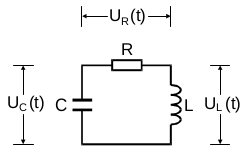
\includegraphics{content/images/V354.png}
  \caption{Gedämpfter L-R-C-Schwingkreis.}
  \label{fig:schwingkreis}
\end{figure}

\begin{equation}
  \symbf{I}_\text{einhüllend} = I_0 e^{-2\pi\mu t} 
\end{equation}
